
\section{Evaluation}\label{sec:evaluation}

In this section, we experimentally analyze various real-time aspects
of the DeepPicar. This includes
(1) measurement based worst-case execution time (WCET) analysis of
deep learning inferencing,
(2) the effect of using multiple cores in accelerating inferencing,
(3) the effect of co-scheduling multiple deep neural network models,
(4) the effect of co-scheduling memory bandwidth intensive co-runners,
and
(5) the effect of partitioning the shared L2 cache.

\subsection{Setup}

The Raspberry Pi 3 Model B platform used in DeepPicar equips a Boardcom
BCM2837 SoC, which has a quad-core ARM Cortex-A53 cluster,
running at up to 1.2GHz. Each core has a 32K private Instruction cache
and a 32K private Data cache, and all cores share a 512KB L2 cache.
The chip also includes Broadcom's Videocore IV
GPU, although we did not use the GPU in our evaluation due to the lack
of sofware support (TensorFlow is not compatible with the Raspberry Pi's GPU).
For software, we use Ubuntu MATE 16.04, TensorFlow 1.1 and Python
2.7. We disabled DVFS (dynamic voltage frequency scaling) and
configured the clock speed of each core statically at the maximum 1.2GHz.

\subsection{Inference Timing for Real-Time Control}

For real-time control of a car (or any robot), the control loop
frequency must be sufficiently high so that the car can quickly
react to the changing environment and its internal states. In general,
control performance improves when the frequency is higher, though
computation time and the type of the particular physical system are
factors in determining a proper control loop frequency. While a standard
control system may be comprised of multiple control loops with
differing control frequencies---e.g., an inner control loop for lower-level
PD control, an outer loop for motion planning, etc.---DeepPicar's
control loop is a single layer, as shown earlier in
Figure~\ref{fig:controlloop}, since a single deep neural network
replaces the traditional multi-layer control pipline. (Refer to
Figure~\ref{fig:end-to-end-control} on the differences between the
standard robotics control vs. end-to-end deep learning approach).
This means that the DNN inference operation must be completed
within the inner-most control loop update frequency. To understand
achievable control-loop update frequencies, we experimentally measured
the execution times of DeepPicar's DNN inference operations.

% 50-200Hz for quadcopters:
% https://robotics.stackexchange.com/questions/231/what-frequency-does-my-quadcopter-output-sense-calculate-output-update-loop-need 
% https://quadmeup.com/pid-looptime-why-it-is-not-only-about-frequency/

\begin{figure}[t]
  \centering
  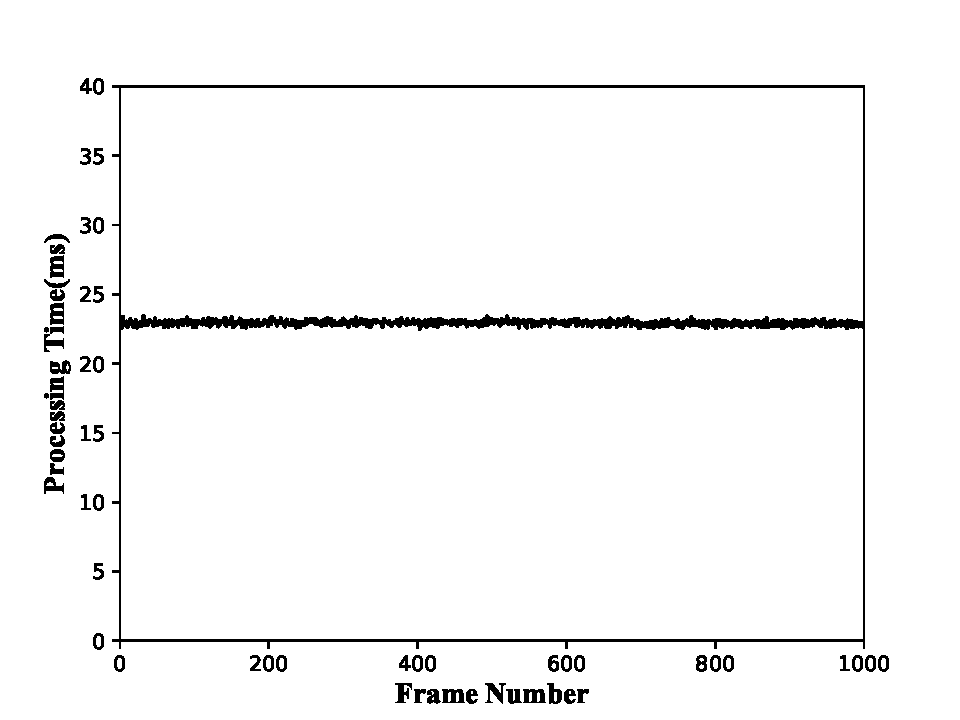
\includegraphics[width=.75\textwidth]{figs/Fig7_new}
  \caption{DeepPicar's control loop processing times over 1000 input image frames.}
  \label{fig:control-loop-timing}
\end{figure}

\begin{table}[t]
  \centering
  \begin{tabular} {| c | r | r | r | r |}
    \hline
    \textbf{Operation} & \textbf{Mean} & \textbf{Max} &   \textbf{99pct.} & \textbf{Stdev.} \\ \hline
    Image capture        & 1.61  &  1.81 &  1.75  & 0.05 \\ \hline
    Image pre-processing & 2.77  &  2.90 &  2.87  & 0.04 \\ \hline
    DNN inferencing      & 18.49 & 19.30 & 18.99  & 0.20 \\ \hline
    Total Time           & 22.87 & 23.74 & 23.38  & 0.20 \\ \hline
  \end{tabular}
  \caption{Control loop timing breakdown.}
  \label{tbl:control-loop-breakdown}
\end{table}

Figure~\ref{fig:control-loop-timing} shows the measured control loop 
processing times of the DeepPicar over 1000 image frames (one per each
control loop). We omit the first frame's processing time for cache
warmup. Table~\ref{tbl:control-loop-breakdown} shows the time
breakdown of each control loop. Note that all four CPU cores of the
Raspberry Pi 3 were used by the TensorFlow library when performing the
DNN inference operations.

First, as expected, we find that the inference operation
dominates the control loop execution time, accounting for about 81\% of
the execution time.

Second, we find that the measured average
execution time of a single control loop is 22.87 ms, or 43.7 Hz and
the 99 percentile time is 23.38 ms.
This means that the DeepPicar can operate
at a up to 40 Hz control frequency in real-time using only the on-board
Raspberry Pi 3 computing platform, as no remote computing resources 
were necessary. We consider these results surprising given the complexity
of the deep neural network, and the fact that the inference operation
performed by TensorFlow only utilizes the CPU cores of the
Raspberry Pi 3 (its GPU is not supported by Tensorflow).
In comparison, NVIDIA's DAVE-2 system, which has the exact same neural
network architecture, reportedly runs at 30 Hz~\cite{Bojarski2016}. 
Although we believe it was not
limited by their computing platform (we will experimentally compare
performance differences among multiple embedded computing platforms,
including NVIDIA's Jetson TX2, later in
Section~\ref{sec:comparison}), the fact that a low-cost
Raspberry Pi 3 can achieve comparable real-time control performance is
surprising.

Lastly, we find that the control loop execution timing is highly
predictable and shows very little variance over different input image
frames. This is because the amount of computation needed to perform
a DNN inferencing operation is fixed at the DNN architecture design
time and does not change at runtime over different inputs (i.e.,
different image frames). This predictable timing behavior is a highly
desirable property for real-time systems, making DNN inferencing an
attractive real-time workload.

\subsection{Effect of the Core Count to Inference Timing}

\begin{figure}[h]
  \centering
  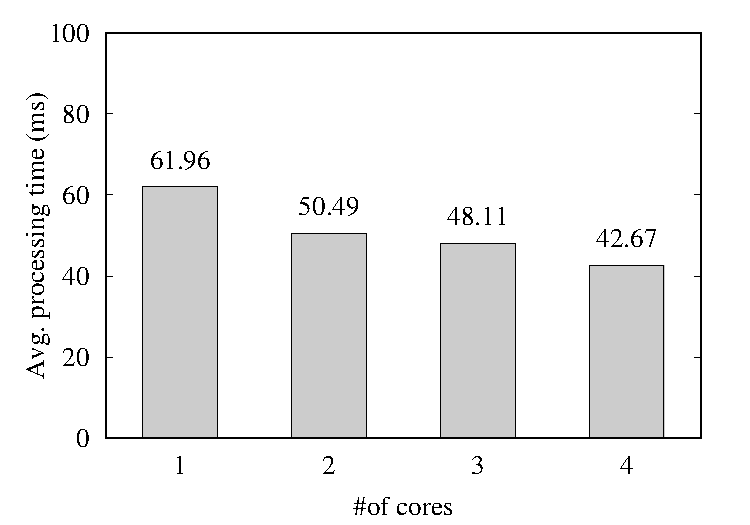
\includegraphics[width=.7\textwidth]{figs/perf_vs_corecnt}
  \caption{Average control loop execution time vs. \#of CPU
    cores.}
  \label{fig:perf-vs-corecnt}
\end{figure}

In this experiment, we investigate the scalability of performing
inference operations of DeepPicar's neural network with respect to the
number of cores. As noted earlier, the Raspberry Pi 3 platform has
four Cortex-A53 cores and TensorFlow 
provides a programmable mechanism to adjust how many cores are to be
used by the library. Leveraging this feature, we repeat the
same experiment described in the previous subsection with varying
numbers of CPU cores---from one to four.

Figure~\ref{fig:perf-vs-corecnt} shows the average execution time of
the control loop as we vary the number of cores used by
TensorFlow. As expected, as we assign more cores, the average execution
time decreases---from 46.30 ms on a single core to 22.86 ms on four
cores (over a 100\% improvement). However, the improvement is far from an ideal
linear scaling. In particular, from 3 cores to 4 cores, the
improvement is mere 2.80 ms, or 12\%. In short, we find that the
scalability of DeepPicar's deep neural network is not ideal on the
platform.

As noted in~\cite{NVIDIA2015}, DNN inferencing is inherently more
difficult to parallelize than training because the easiest
parallelization option, batching (i.e., processing multiple images in
parallel), is not available or is limited. Specifically, in DeepPicar,
only one image frame, obtained from the camera, can be processed at a
time. Thus, more fine-grained algorithmic parallelization is needed to
improve inference performance~\cite{NVIDIA2015}, which generally does
not scale very well. 

On the other hand, the poor scalability opens up the possibility of
consolidating multiple different tasks or different neural network
models rather than allocating all cores for a single neural network
model.
For example, it is conceivable to use four cameras and four different
neural network models, each of which is trained separately for
different purpose and executed on a single dedicated core.
Assuming we use the same network
architecture for all models, then one might expect to achieve up to
20 Hz using one core (given 1 core can deliver 46 ms average
execution time).
In the next experiment, we investigate the
feasibility of such a scenario.

\subsection{Effect of Co-scheduling Multiple DNN Models}

In this experiment, we launch multiple instances of DeepPicar's DNN
model at the same time and measure its impact on their inference
timings. In other words, we are interested in how shared resource
contention affects inference timing. These instances are not identical
copies of the same model, but are instead copies of different models. 
This is done to ensure that no L2 cache memory is shared between the 
models as they are running.

\begin{figure}[h]
  \centering
  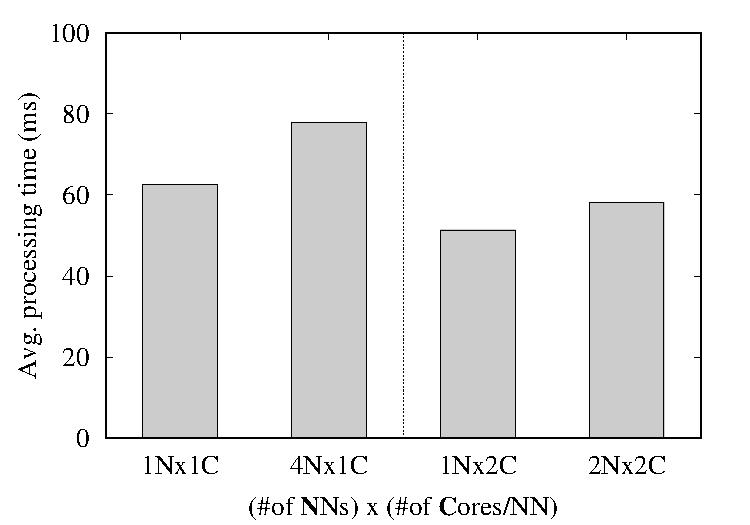
\includegraphics[width=.7\textwidth]{figs/perf_vs_modelcnt}
  \caption{Timing impact of co-scheduling multiple DNNs. 1Nx1C: one DNN
    model using one core; 4Nx1C: four DNN models each using one core;
    1Nx2C: one DNN model using two cores; 2Nx2C: two DNN models each
    using two cores.} 
  \label{fig:perf-vs-modelcnt}
\end{figure}

Figure~\ref{fig:perf-vs-modelcnt} shows the results. In the figure, the
X-axis shows the system configuration: \#of DNN models x \#of CPU
cores/DNN. For example, '4Nx1C' means running four DNN models each of
which is assigned to run on one CPU core, whereas '2Nx2C' means running
two DNN models, each of which is assigned to run on two CPU
cores. The Y-axis shows the average inference timing.
The two bars on the left show the impact of co-scheduling four DNN
models. Compared to executing a single DNN model on one CPU core
(1Nx1C), when four DNN models are co-scheduled (4Nx1C), each model
suffers an average inference time increase of approximately 11 ms,
$\sim$24\%. On the other hand, when two DNN models, each using two CPU
cores, are co-scheduled (2Nx2C), the average inference timing is increased by
about 4 ms, or 13\%, compared to the baseline of running one model
using two CPU cores (1Nx2C). 

These increases in inference times in the co-scheduled scenarios are
expected and are caused by contention in the shared hardware
resources, such as the shared L2 cache and/or the DRAM controller.

%% \begin{figure}[h]
%%   \centering
%%   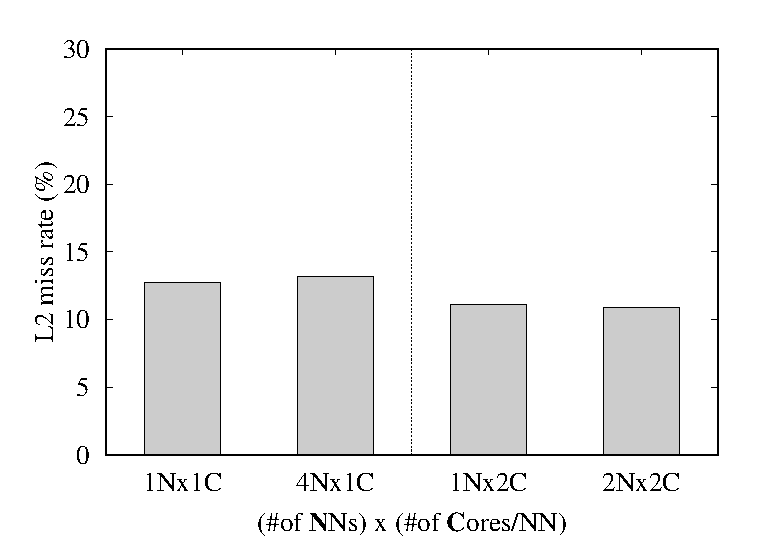
\includegraphics[width=.7\textwidth]{figs/l2missrate_vs_modelcnt}
%%   \caption{L2 cache miss rates of different neural network and core
%%     assignments. X-axis is the same as Figure~\ref{fig:perf-vs-modelcnt}.} 
%%   \label{fig:l2missrate-vs-modelcnt}
%% \end{figure}

%% To further analyze the source of contention, we use hardware
%% performance counters of the processor. Specifically, we measure L2
%% miss rates of the DNN models first in isolation and then after
%% co-scheduling other models. If the shared L2 cache is the primary
%% source of inteference, then the measured L2 miss rates will
%% increase. Figure~\ref{fig:l2missrate-vs-modelcnt} shows the results.
%% As can be see in the figure, L2 miss rates increase as more models are 
%% co-scheduled, but the increase is less than expected.
%% This suggests that the shared L2 cache is not the main bottleneck that 
%% causes execution time increases. In other words, DNN models don't appear 
%% to be significantly affected by the shared L2 cache space. 
%% % L2 partitioning is probably not going to be useful.
%% Instead, we hypothesize that it is likely caused by the memory
%% controller---the only other major shared hardware source---where
%% memory requests from different CPU cores contend, which would result
%% in increased memory access latency. While some Intel processors
%% provide incore hardware counters that can measure average memory
%% access latency~\cite{ye2016maracas}, we were not able to identify
%% whether such hardware counters exist in the BCM2837 processor of
%% Raspberry Pi 3 due to the lack of documentation. Instead, in the next
%% experiment, we use memory intensive synthetic benchmarks to test the
%% hypothesis.

\subsection{Effect of Co-scheduling Memory Performance Hogs}\label{sec:eval-memhog}

In this experiment, we investigate the impact of contended DRAM
requests to the DNN inference timing of DeepPicar.
For the experiment, we use a synthetic memory
intensive benchmark from the IsolBench suite~\cite{Valsan2016}.
We run a single DNN model on one core, and
co-schedule an increasing number of the memory intensive synthetic
benchmarks~\footnote{We use the \emph{Bandwidth} benchmark in the
  IsolBench suite, with the following command line parameters: \texttt{\$
  bandwdith -a write -m 16384}}, on the remaining idle cores.

\begin{figure}[h]
  \centering
  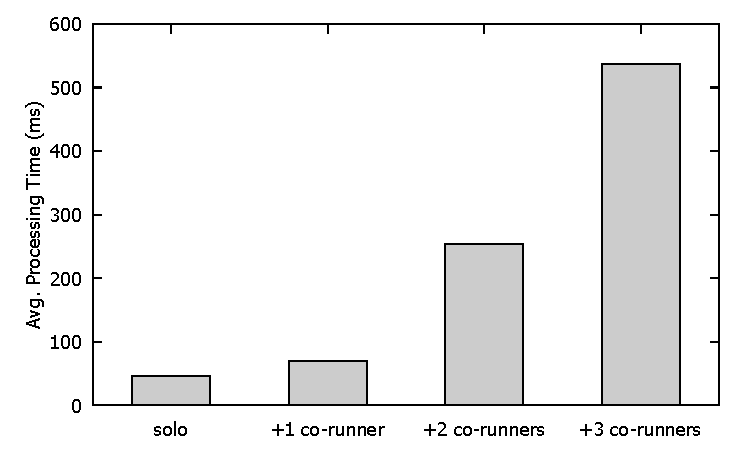
\includegraphics[width=.7\textwidth]{figs/perf_vs_bandwidth}
  \caption{Effect of memory performance hogs on the DNN
    inferencing. The DNN model uses Core 0 and memory-hog co-runners
    use the rest of the cores.}
  \label{fig:}
\end{figure}

Figure~\ref{fig:} shows the normalized execution time and L2 miss-rate
of the DNN model running on the Core 0 as a function of the number of
co-scheduled memory intensive synthetic benchmarks. First, as we
increase the number of co-runners, the DNN model's execution times are
increased---by up to 11.6X---even though the DNN model is running on a
dedicated core (Core 0). On the other hand, the DNN model's L2
cache-miss rates do not increase as much.
In other words, the DNN model's execution increase is not fully
explained by increased contention in the L2 cache space.
Instead, the high memory bandwidth pressure from the co-scheduled
memory intensive benchmarks is likely the primary cause.

%% Instead, as we hypothesized in the previous
%% experiment, the increased memory pressure from the co-scheduled memory
%% intensive benchmarks is likely the primary cause of the DNN model's execution
%% time increase. Therefore, we conclude that DeepPicar's DNN model is
%% more senstive to DRAM access latency than L2 cache space.

This observation suggests that shared cache partitioning
techniques~\cite{Gracioli2015,Kim2016} may not be effective isolation
solutions for DeepPicar's DNN processing workload, as cache
partitioning does not provide memory performance guarantees.

%% Instead, memory controller focused isolation solutions,
%% either hardware or software-based ones (e.g.,~\cite{Guo2017,Yun2013}),
%% may be more important. Although our observation is made on a single
%% hardware platform running on a single DNN workload, we suspect that
%% many AI workloads may exhibit similar characteristics.

% \subsection{Effect of Cache Partitioning}

%% \begin{figure}[h]
%%   \centering
%%   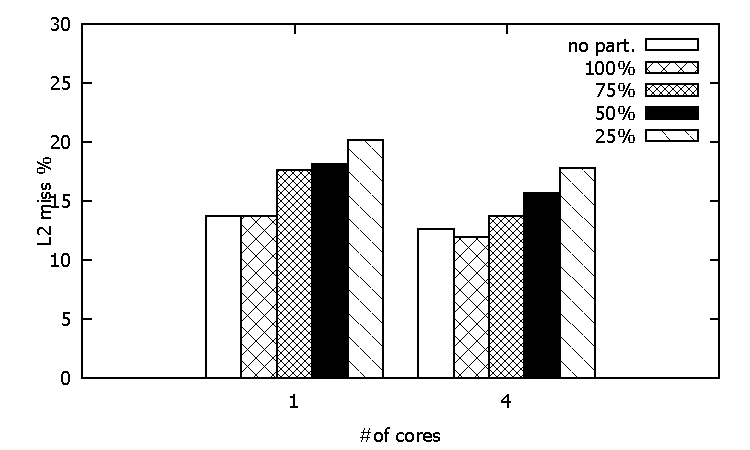
\includegraphics[width=.7\textwidth]{figs/palloc_multicore_l2missrate}
%%   \caption{L2 miss rate impact of limiting the amount of L2 cache space
%%   available to the DNN.}
%%   \label{fig:palloc_multicore_l2missrate}
%% \end{figure}

%% \begin{figure}[h]
%%   \centering
%%   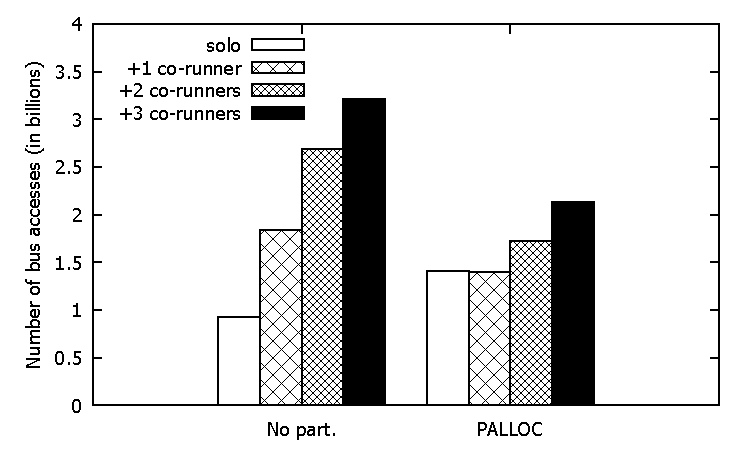
\includegraphics[width=.7\textwidth]{figs/palloc_bandwidth_modelbus}
%%   \caption{Model bus access impact of co-scheduling memory intensive co-runners 
%% when cache partitioning is enabled.}
%%   \label{fig:palloc_bandwidth_modelbus}
%% \end{figure}

%% \begin{figure}[h]
%%   \centering
%%   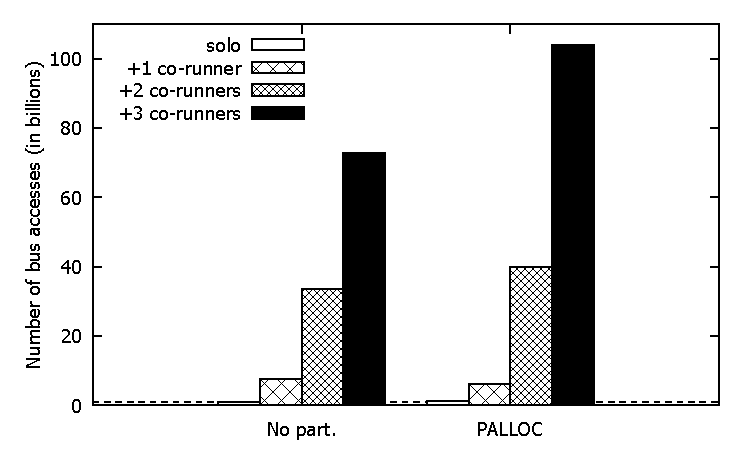
\includegraphics[width=.7\textwidth]{figs/palloc_bandwidth_bus}
%%   \caption{Total bus access impact of co-scheduling memory intensive co-runners 
%% when cache partitioning is enabled.}
%%   \label{fig:palloc_bandwidth_bus}
%% \end{figure}

%% \begin{figure}[h]
%%   \centering
%%   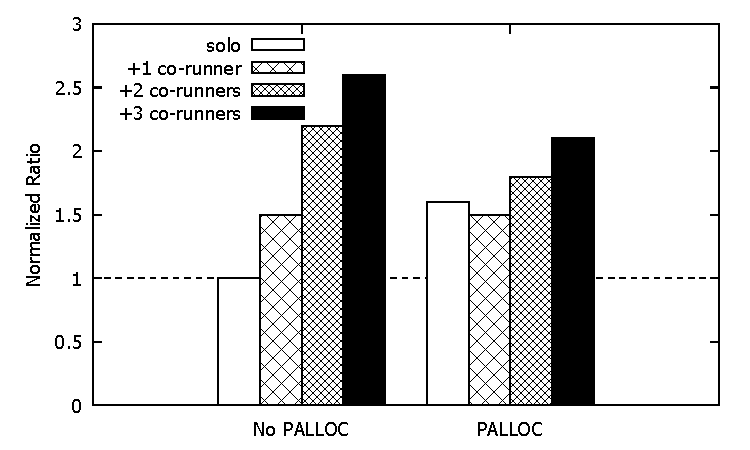
\includegraphics[width=.7\textwidth]{figs/palloc_bandwidth_l2missrate}
%%   \caption{L2 miss rate impact of co-scheduling memory intensive co-
%% runners when cache partitioning is enabled.}
%%   \label{fig:palloc_bandwidth_l2missrate}
%% \end{figure}

Cache partitioning is a well-known technique to improve isolation in
real-time systems by giving a dedicated cache space to each individaul
task or core. In this experiment, we use PALLOC~\cite{yun2014rtas}, a
page-coloring based cache partitioning solution for Linux, to
investigate the effect of cache partitioning in protecting DeepPicar's
DNN based controller.

\begin{figure}
  \centering
  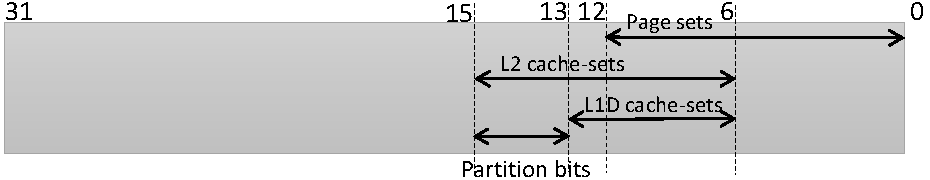
\includegraphics[width=.5\textwidth]{figs/cache-mapping}
  \caption{Physical address mapping of L1/L2 caches of Broadcom
    BCM2837 processor in Raspberry Pi 3.}
  \label{fig:cache-mapping}
\end{figure}

Page coloring is a OS technique that controls the physical addresses
of memory pages. By allocating pages over non-overlapping sets of the
cache, the OS can effectively partition the cache.
Figure~\ref{fig:cache-mapping} shows the physical address
mapping of Raspberry Pi 3's BCM2837 processor, which has 32K private
L1 I\&D (4way) caches and a share 512KB L2 (16 way) cache. In order not
to partition the private L1 caches, we use the bit 13 and 14 for
coloring, which results in 4 usuable page colors.

%% determine if the DNN is mostly affected by the DRAM 
%% controller, we partition the L2 cache of the Pi3 and reperform the 
%% same experiments to see if there are any noticable changes. For the 
%% partition, we employ PALLOC~\cite{yun2014rtas}, a color-based page 
%% allocator that works on the kernel level.

%% For the bit mask, we select 
%% bits 12, 13 and 14 as they can be used to access the L2 cache,
%% as can be seen by Figure \ref{fig:cache-mapping}.
%% This results in 
%% 2\textsuperscript{3} = 8 colors, which we then assign to the Pi3's 
%% physical cores such that each core has two unique colors (colors 0 
%% and 1 are assigned to core 0, colors 2 and 3 are assigned to core 1, 
%% etc.). In the case of bit 12, since we use 2 colors for each partition,
%% the L1 Data cache is not partitioned in our experiments.

\begin{figure}[h]
  \centering
  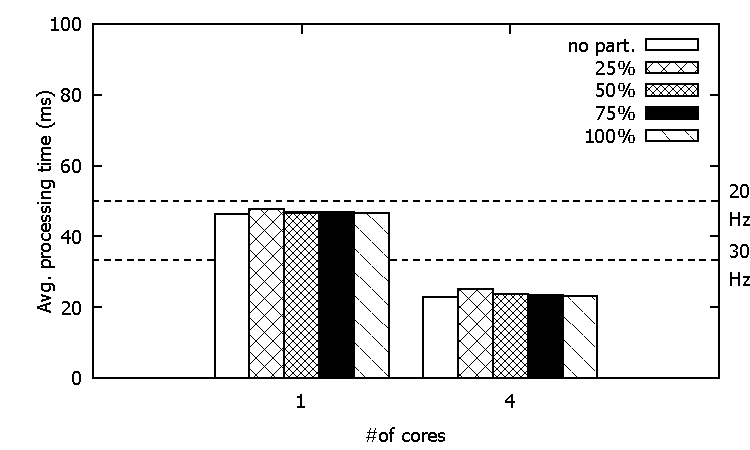
\includegraphics[width=.45\textwidth]{figs/palloc_multicore}
  \caption{Cache space sensitivity of the DNN controller. \fixme{I
      think 'no part.' bar is not necessary here.}}
  \label{fig:palloc_multicore}
\end{figure}

In the first experiment, we investigate the cache space sensitivity of
DeepPicar's DNN-based control loop. Using PALLOC, we create 4
different cgroups which are configured to use 4, 3,
2, and 1 colors (100\%, 75\%, 50\% and 25\% of the L2 cache
space, respectively). We then execute the DNN control loop (inference)
on each cache partition (cgroup) and measure the average processing
time.

Figure~\ref{fig:palloc_multicore} shows the result. As can be seen,
the DNN inference timing is hardly changed at all regardless of the
size of the allocated L2 cache space. In other words, we find that
the DNN workload is largely insensitive to L2 cache space.

The next experiment further validates this finding. In this
experiment, we repeat the experiment in
Section~\ref{sec:eval-memhog}---i.e., co-scheduling the DNN model and
three Bandwidth (BwRead or BwWrite) instances---but this time we
ensure that each task is given equal amounts of L2 cache space by
assigning one color to each task's cache partition.

\begin{figure}[h]
  \centering
  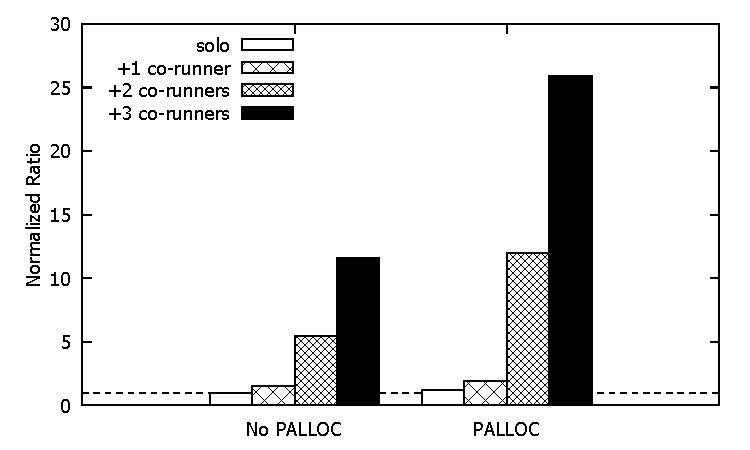
\includegraphics[width=.45\textwidth]{figs/palloc_bandwidth_exectime}
  \caption{Average processing time vs. the number of memory
memory intensive co-runners. Unlike
Figure~\ref{fig:perf_vs_bandwidth}, the shared L2 cache is equally
partitioned and each task is given a dedicated cache
partition. \fixme{how about changing the figure style to be the same
  as Figure 9.}}
  \label{fig:palloc_bandwidth_exectime}
\end{figure}

Figure \ref{fig:palloc_bandwidth_exectime} shows the
result. For BwRead, when cache partitioning is enabled, DNN
performance becomes slightly better, with a improvement of  
\textasciitilde6.5\%. For BwWrite, cache partitioning actually makes
the DNN performance slightly worse that that of w/o partitioning.

In summary, we find that the DNN inferencing workload is not sensitive
to cache space and that cache partitioning is not effective in
providing timing isolation to our DNN workload.

%% By partitioning the shared L2 cache, we find that no noticable 
%% improvements are gained and that performance remains consistent. 
%% In all experiements, the model shows no sensitivity to the shared L2 
%% cache. As a result, we conclude that cache partitioning is not an 
%% effective isolation mechanism, and that the performance of the shared 
%% DRAM controller is of greater importance to the real-time efficiacy of 
%% the DeepPicar.

%% If performance improves as a result of partitioning the shared cache 
%% then we know that the DNN, to some extent, relies on the shared cache 
%% in addition to the shared DRAM. On the other 
%% hand, if there is no improvement in performance, then it can be 
%% observed that the shared memory is more critical for the DNN.

%% We run the DNN model with different amounts of L2 cache being
%% available based on the number of colors being used. For example, if two 
%% colors are used, then 25\% of the L2 cache is available, whereas if all 
%% 8 colors are used, 100\% of the L2 cache is available. Particularly, we 
%% test the performance of the model when it utilizes a single core and
%% all four of the available cores. 

%% As expected, the amount of L2 cache 
%% available to the model does not result in any significant changes in 
%% performance. 
%% This can also be seen by the L2 miss rates of the model 
%% seen in \ref{fig:palloc_multicore_l2missrate}. As more cache space 
%% becomes avaiable, the percentage of L2 misses decreases, which doesn't 
%% affect the real-time performance of the DNN. As such, we find that a 
%% single model is not sensitive to the shared L2 cache.

%% \begin{figure}[h]
%%  \centering
%%   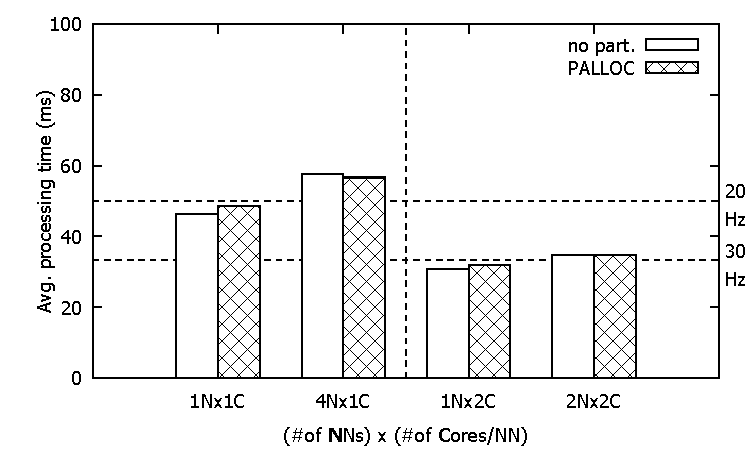
\includegraphics[width=.45\textwidth]{figs/palloc_multimodel}
%%   \caption{Timing impact of co-scheduling multiple DNNs when cache 
%% partitioning is enabled.}
%%   \label{fig:palloc_multimodel}
%% \end{figure}

%% We also co-schedule multiple models to see how cache partitioning affects
%% interference between them. Each model uses an equal number of colors, and
%% are thus given equal amounts of L2 cache space, and there is no overlap
%% in the colors used, so no L2 cache is shared between models. As can be 
%% seen in Figure \ref{fig:palloc_multimodel}, the performance of the models 
%% remains the same as when no cache partitioning was employed. Based of 
%% these results, we find that contention for the L2 cache is not the main
%% source of interference between multiple DNN models.

%% At the same time, though, the L2 miss rates of the model don't correlate 
%% to the timing increases seen, as is shown in 
%% \ref{fig:palloc_bandwidth_l2missrate}. Instead, we find that the number
%% of bus accesses increases when cache partitions are used, and they mirror
%% the timing increases of the model. This can be seen in Figure 
%% \ref{fig:palloc_bandwidth_bus}. These additional bus accesses are
%% most likely caused by the L2 prefetcher, as it can generate additional bus
%% accesses that aren't counted as L2 misses. As a result, we find that cache
%% partitioning is detrimental to the performance of the DNN so long as the 
%% 0L2 prefetcher is enabled (we have not yet found a way to disable it on
%% the Pi 3). Furthermore, no cache sensitivity was displayed by the model,
%% thus showing that the performance of the L2 cache is not vital for DNN 
%% performance when co-runners are introduced.



\subsection{Summary of the Findings}
So far, we have evaluated DeepPicar's real-time
characteristics from the perspective of end-to-end deep learning based
real-time control, and made several observations.

First, we find that DeepPicar's computing platform,
the Raspberry Pi 3 Model B, offers computing capacity to
perform real-time control of the RC car at 30 Hz frequency (or
33.$\overline{\mbox{33}}$ ms  per control loop). Given the complexity of 
the DNN used, we were pleasantly surprised by this finding. 
The time breakdown shows that the DNN inferencing operation, 
performed by the Tensorflow library, dominates the execution time, 
which is expected.

Second, we find that scalability of Tensorflow's DNN 
implementation is limited. We find that using all four cores can double 
performance of the DNN, but compared to using three cores, performance
improvement is relatively minimal.

Third, we find that consolidating multiple DNN models---on different CPU
cores---is feasible as we find: (1) DNN performance using a single
core is not much worse than using multiple cores; (2) multiple DNN
models running simultaneously do not cause severe interference with
each other.

Fourth, we find that consolidating memory (DRAM) performance
intensive applications could jeopadize DNN performance, because DNN
performance appears to be very sensitive to memory performance; we 
observe up to 11.6X slowdown in DNN performance by co-scheduling 
synthetic memory bandwidth intensive applications on idle cores.

%% Lastly, we find that partitioning the shared L2 cache provides 
%% practically no benefits to the real-time performance of the DNN. To the 
%% contrary, performance is constant regardless of the amount of cache 
%% space used. We also find that performance becomes worse when memory
%% intensive co-runners are introduced as they generate more memory 
%% contention when partitioning is enabled. Furthermore, we 
%% find that performance remains consistent when multiple models are run 
%% simultaneously. As such, we conclude that the shared L2 cache is not 
%% essential to the DNN's real-time performance.
